\section{Hiện thực}
Chương này tập trung trình bày các giải pháp công nghệ và hạ tầng kỹ thuật được áp dụng để hiện thực hóa và triển khai hệ thống. Việc lựa chọn các công nghệ này đóng vai trò quyết định đến tính ổn định trong vận hành, đồng thời đảm bảo khả năng đáp ứng trọn vẹn các yêu cầu đã được đề ra.

\subsection{Công nghệ sử dụng}
\subsubsection{Giao diện người dùng}

\begin{itemize}
  \item \textbf{Next.js (React)}
    \begin{itemize}
      \item \textbf{Giới thiệu:} Next.js là một framework React mã nguồn mở được phát triển bởi Vercel, hỗ trợ rendering phía server (SSR) và tạo trang tĩnh (SSG) \cite{nextjsdocs}.
      \item \textbf{Lý do sử dụng:} Next.js có khả năng tối ưu hiệu năng với Server-Side Rendering và Static Site Generation, giúp trang web load nhanh và thân thiện với SEO, ngoài ra framework này còn hỗ trợ routing tự động, API routes tích hợp sẵn, và có hệ sinh thái React phong phú với nhiều thư viện UI component \cite{nextjsdocs}. Next.js cho phép phát triển full-stack với cả frontend và backend API trong cùng một dự án, giúp đơn giản hóa quá trình phát triển. Ngoài ra, việc triển khai lên Vercel hoặc các nền tảng cloud khác rất dễ dàng, có cộng đồng hỗ trợ lớn và được cập nhật thường xuyên. Nhược điểm chính là learning curve cao hơn so với React thuần, nhưng đổi lại mang lại hiệu năng và trải nghiệm người dùng vượt trội.
    \end{itemize}
    
  \item \textbf{Cocos Creator}
    \begin{itemize}
      \item \textbf{Giới thiệu:} Cocos Creator là một game engine đa nền tảng mã nguồn mở, chuyên dụng cho phát triển game 2D/3D và các ứng dụng tương tác \cite{cocoscreator38}.
      \item \textbf{Lý do sử dụng:} Cocos Creator được sử dụng để tạo các bài tập tương tác (interactive exercises) và minigames với đồ họa phong phú, animation mượt mà. Engine này hỗ trợ export ra WebGL để chạy trực tiếp trên trình duyệt web, tích hợp dễ dàng với Next.js. Cocos Creator cung cấp editor trực quan giúp thiết kế game nhanh chóng, hỗ trợ physics engine tích hợp sẵn, và có khả năng xử lý nhiều đối tượng game cùng lúc với hiệu năng cao \cite{cocoscreator38}. Điều này rất phù hợp cho việc tạo các trò chơi toán học tương tác, bài tập kéo thả, và các minigame giáo dục hấp dẫn.
    \end{itemize}

  \item \textbf{Colyseus}
    \begin{itemize}
      \item \textbf{Giới thiệu:} Colyseus là một framework mã nguồn mở chuyên dụng cho việc xây dựng máy chủ game đa người chơi thời gian thực (real-time multiplayer), được phát triển trên nền tảng Node.js và sử dụng giao thức WebSocket để truyền tải dữ liệu hai chiều với độ trễ thấp.
      \item \textbf{Lý do sử dụng:} Trong hệ thống Dino Math, Colyseus được tích hợp để hỗ trợ tính năng minigame tương tác giữa hai người chơi, cụ thể là minigame \textbf{Tomato Shooting} -- trò chơi đối kháng thời gian thực lấy ý tưởng từ Gunny, trong đó hai người chơi cạnh tranh trả lời các phép tính toán học bằng cách bắn trúng đáp án đúng trước đối thủ. Colyseus cung cấp cơ chế quản lý \textit{Room} (phòng chơi) cho phép nhóm nhiều người chơi vào cùng một phiên game, đồng bộ hóa trạng thái game (game state) giữa tất cả các client thông qua \textit{Schema} -- một cấu trúc dữ liệu được tối ưu để chỉ truyền phần dữ liệu thay đổi (delta), giảm thiểu băng thông. Client Colyseus được tích hợp trực tiếp vào Cocos Creator thông qua SDK chính thức, giúp việc đồng bộ trạng thái game giữa server và engine trở nên liền mạch. Bên cạnh đó, Colyseus hỗ trợ cơ chế \textit{matchmaking} đơn giản, cho phép tự động ghép cặp hai người chơi vào cùng một phòng, cũng như xử lý các tình huống ngắt kết nối và tái kết nối (reconnect) một cách graceful.
    \end{itemize}
\end{itemize}


\subsubsection{Công nghệ Backend và Quản lý dữ liệu}
\begin{itemize}
	\item \textbf{Node.js \& Express.js}
	\begin{itemize}
		\item \textbf{Giới thiệu:} Node.js là một môi trường thực thi JavaScript phía server dựa trên V8 engine của Chrome, trong khi Express.js là một framework ứng dụng web tối giản, linh hoạt chạy trên nền tảng Node.js \cite{nodejs, expressjs}.
		\item \textbf{Lý do sử dụng:} Sự kết hợp giữa Node.js và Express.js cho phép xây dựng các dịch vụ API có hiệu suất cao nhờ cơ chế hướng sự kiện (event-driven) và I/O không chặn (non-blocking I/O). Điều này đặc biệt quan trọng đối với các tính năng thời gian thực trong Đấu trường, nơi cần xử lý đồng thời nhiều kết nối từ học sinh. Theo tài liệu chính thức \cite{expressjs}, Express.js cung cấp hệ thống Middleware mạnh mẽ, giúp nhóm dễ dàng quản lý luồng dữ liệu, xác thực người dùng và tích hợp các dịch vụ bên thứ ba một cách nhất quán. Việc sử dụng ngôn ngữ TypeScript đồng bộ từ Frontend đến Backend giúp giảm thiểu sai sót về kiểu dữ liệu và tăng tốc độ phát triển dự án.
	\end{itemize}
	
	\item \textbf{MongoDB} 
	\begin{itemize}
		\item \textbf{Giới thiệu:} MongoDB là hệ quản trị cơ sở dữ liệu NoSQL hướng tài liệu (document-oriented), lưu trữ dữ liệu dưới dạng các tài liệu có cấu trúc tương tự JSON \cite{mongodb}.
		\item \textbf{Lý do sử dụng:} MongoDB đóng vai trò là cơ sở dữ liệu chính để lưu trữ thông tin người dùng, kho câu hỏi, kết quả học tập và dữ liệu thống kê. Với tính chất \textit{schema-less}, MongoDB cho phép lưu trữ các định dạng câu hỏi toán học đa dạng (kéo thả, trắc nghiệm, điền số) mà không cần cấu trúc bảng cứng nhắc. Hệ thống tận dụng Mongoose ODM để giao tiếp giữa Node.js và cơ sở dữ liệu, giúp quản lý dữ liệu chặt chẽ hơn qua các định nghĩa Schema. Ngoài ra, khả năng mở rộng ngang (horizontal scaling) và Aggregation Pipeline mạnh mẽ của MongoDB hỗ trợ hiệu quả cho việc xử lý các truy vấn phức tạp như tính toán độ chính xác trung bình và thống kê lịch sử làm bài của học sinh.
	\end{itemize}
	
	\item \textbf{Redis} 
	\begin{itemize}
		\item \textbf{Giới thiệu:} Redis là hệ thống lưu trữ dữ liệu cấu trúc key-value dưới dạng in-memory (lưu trữ trên RAM), thường được dùng làm bộ nhớ đệm (caching) \cite{redis}.
		\item \textbf{Lý do sử dụng:} Redis được tích hợp để tối ưu hóa tốc độ phản hồi của hệ thống thông qua việc lưu trữ các dữ liệu có tần suất truy cập cao nhưng ít thay đổi hoặc các dữ liệu mang tính tạm thời như phiên đăng nhập (session). Đặc biệt, trong tính năng Đấu trường, Redis hỗ trợ tính toán và hiển thị bảng xếp hạng (leaderboard) theo thời gian thực với độ trễ cực thấp, mang lại trải nghiệm mượt mà cho học sinh khi tham gia thi đấu.
	\end{itemize}
\end{itemize}

\newpage
\subsubsection{Dịch vụ bên ngoài}
\begin{itemize}
  \item \textbf{Payment Gateway}
    \begin{itemize}
      \item \textbf{Giới thiệu:} Dịch vụ thanh toán trực tuyến của bên thứ ba (VNPay).
      \item \textbf{Lý do sử dụng:} Xử lý các giao dịch thanh toán cho việc đăng ký Premium một cách an toàn và tuân thủ các tiêu chuẩn bảo mật PCI DSS. Hỗ trợ nhiều phương thức thanh toán phổ biến tại Việt Nam như chuyển khoản ngân hàng, QR code, và ví điện tử. Cung cấp webhook để cập nhật trạng thái thanh toán real-time.
    \end{itemize}
    \item \textbf{Gmail}
    \begin{itemize}
    	\item \textbf{Giới thiệu:} Dịch vụ thư điện tử phổ biến hiện nay của Google.
    	\item \textbf{Lý do sử dụng:} Hỗ trợ việc xác thực danh tính người dùng bằng cách gửi mã xác thực qua email, được dùng cho tính năng đổi hoặc khôi phục mật khẩu.
    \end{itemize}
    \item \textbf{Google OAuth 2.0}
    \begin{itemize}
    	\item \textbf{Giới thiệu:} Cơ thức ủy quyền bảo mật cho phép người dùng chia sẻ tài liệu hoặc quyền truy cập từ tài khoản Google của mình cho các ứng dụng khác mà không cần tiết lộ mật khẩu cá nhân.
    	\item \textbf{Lý do sử dụng:} Được sử dụng cho tính năng đăng nhập vào hệ thống bằng tài khoản Google (dành cho phụ huynh).
    \end{itemize}
 \end{itemize}
 
 \subsubsection{Quản lý mã nguồn}

 \begin{itemize}
 	\item \textbf{Giới thiệu:} GitHub là nền tảng quản lý mã nguồn dựa trên Git, hỗ trợ cộng tác phát triển phần mềm trên phạm vi toàn cầu \cite{github}.
 	\item \textbf{Lý do sử dụng:} Là dịch vụ tiêu chuẩn trong việc lưu trữ mã nguồn, theo dõi lịch sử thay đổi (version control), thực hiện quy trình kiểm tra mã (code review) và tích hợp linh hoạt với các công cụ CI/CD của bên thứ ba.
 \end{itemize}

\subsection{Triển khai hệ thống}
Dưới đây là lược đồ triển khai (Deployment Diagram) tổng thể của hệ thống. Sơ đồ mô tả sự phân bổ các thành phần phần mềm trên hạ tầng đa nền tảng (Vercel, AWS, Render, GitHub Pages) , đồng thể hiện các luồng giao tiếp và giao thức kết nối giữa các dịch vụ nhằm đảm bảo tính vận hành ổn định và hiệu quả.

\begin{figure}[H]
	\centering
	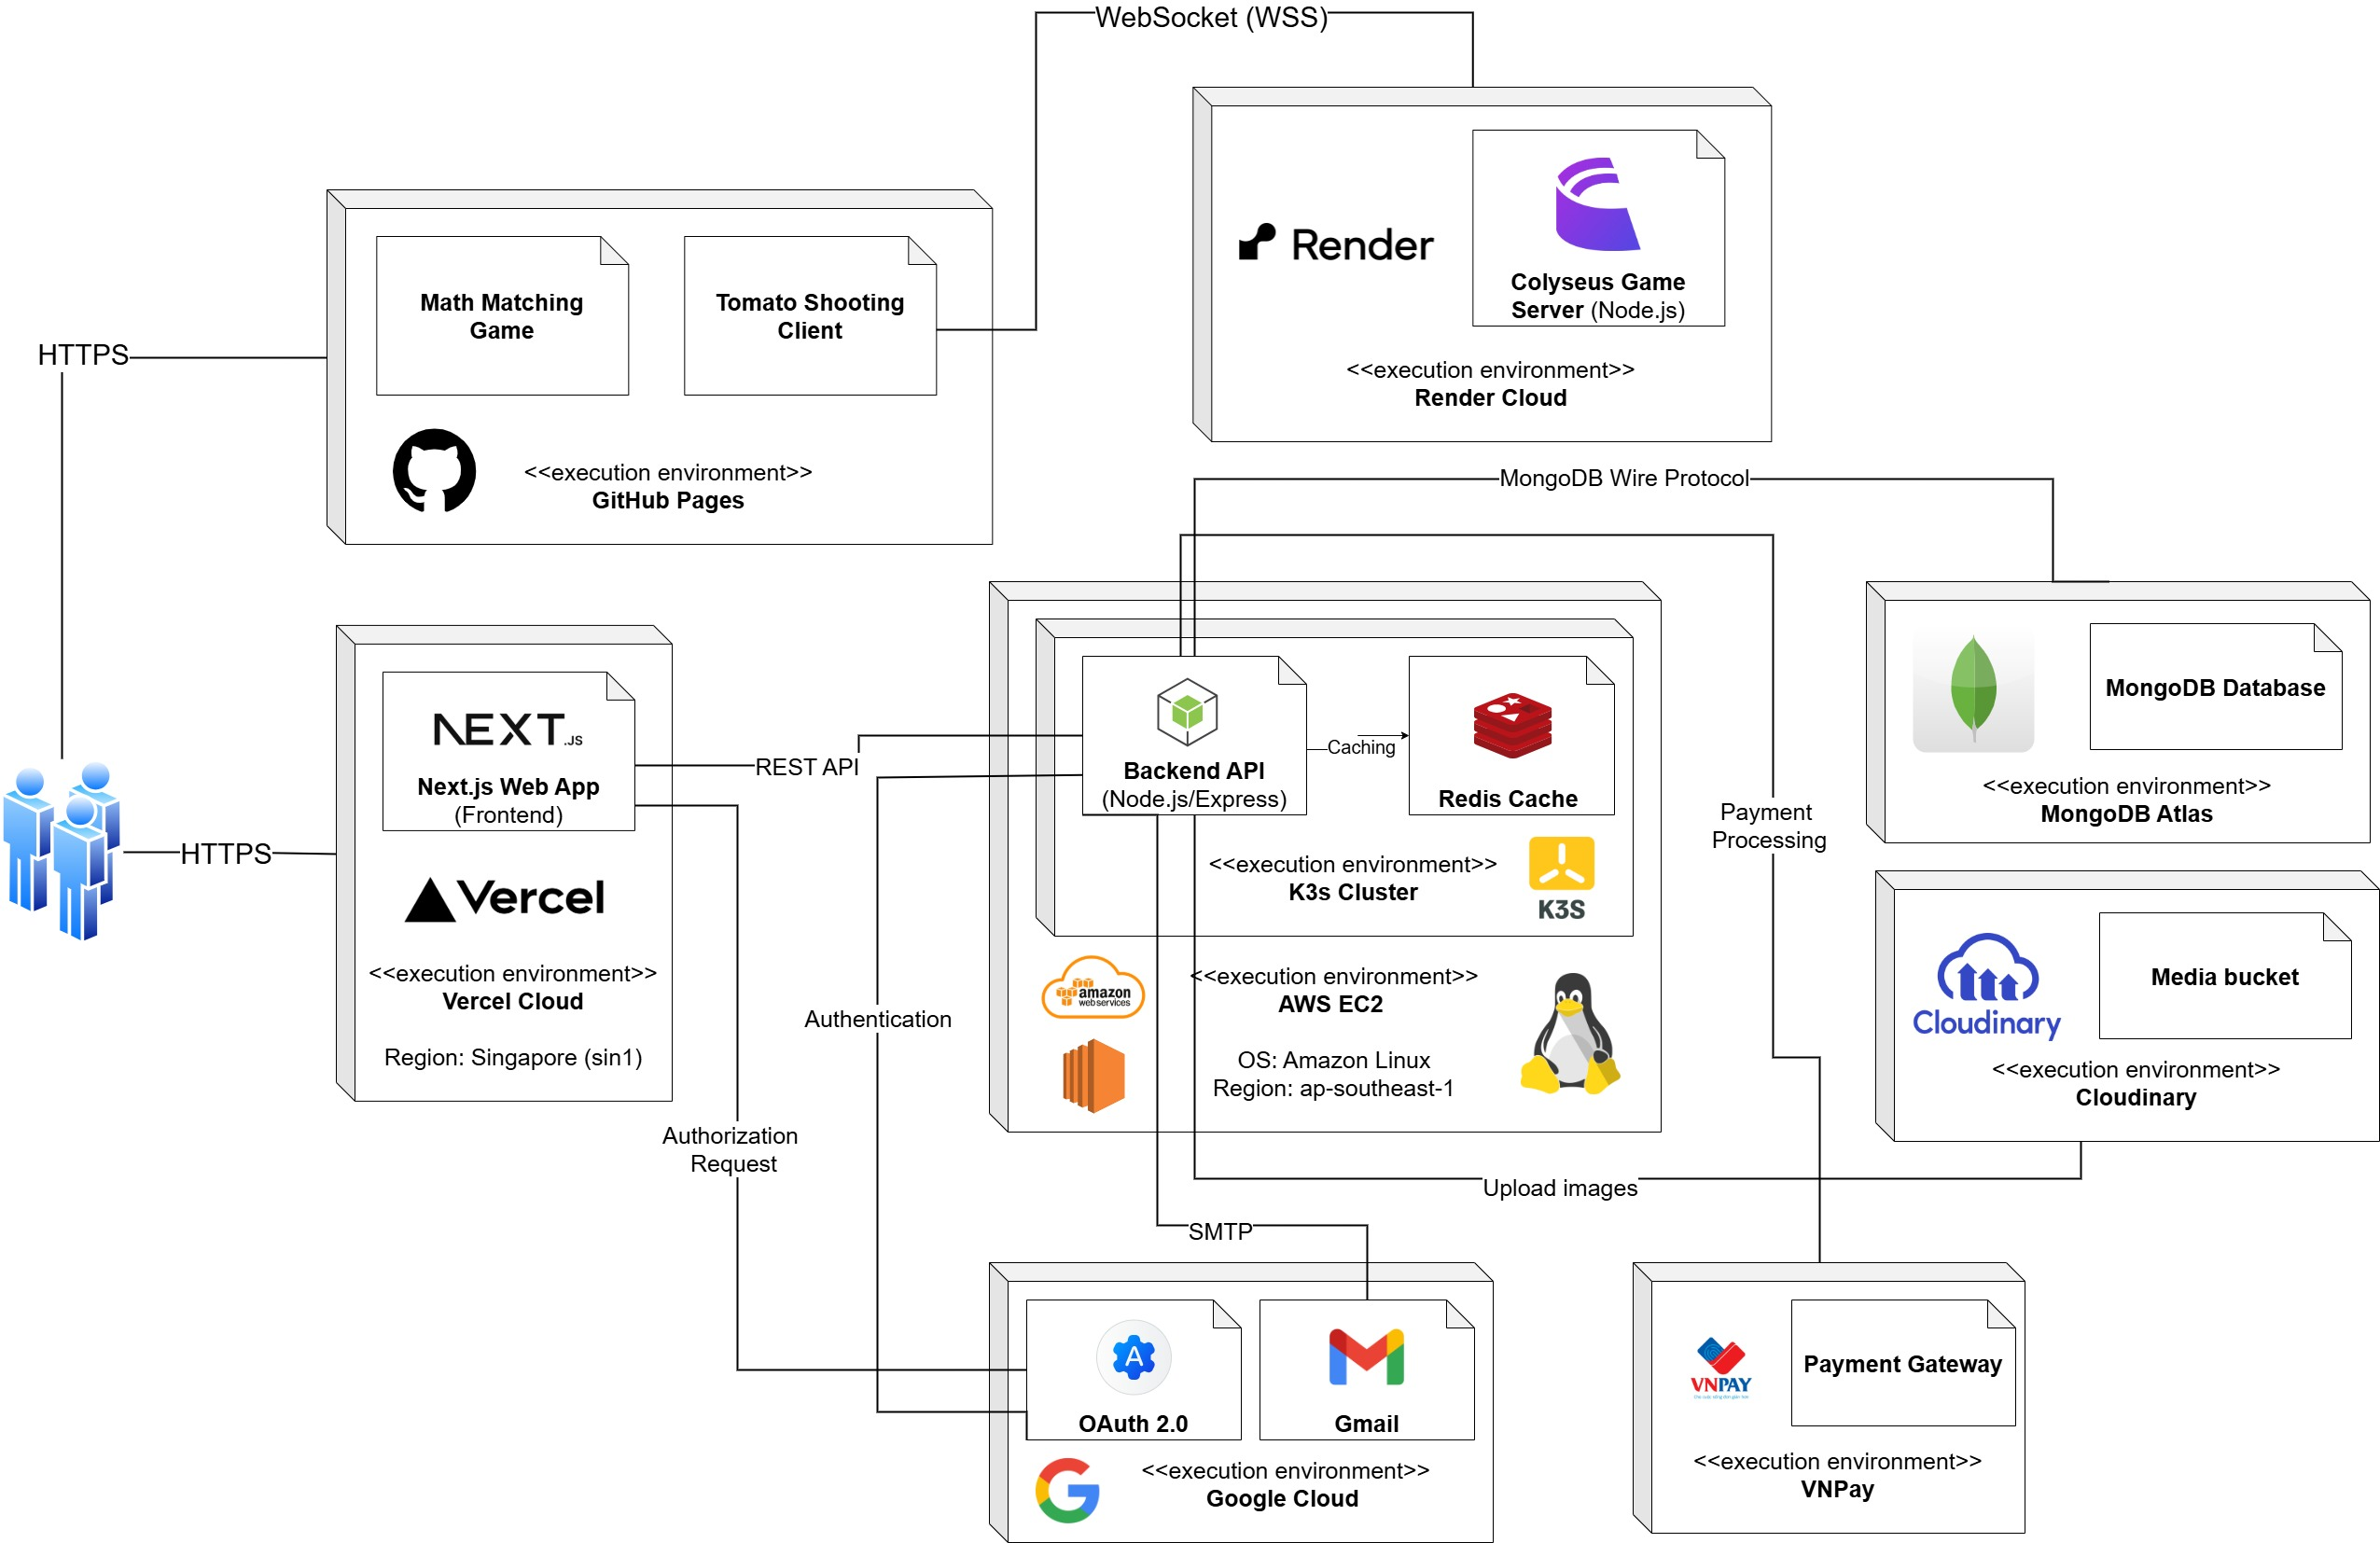
\includegraphics[width=1.0\textwidth]{Image/Deployment.jpg}
	\vspace{0.6cm}
	\caption{Landing Page}
	\label{fig:deploy}
\end{figure}

\subsubsection{Giao diện người dùng (Frontend)}
Giao diện người dùng được triển khai trên nền tảng điện toán đám mây Vercel được tối ưu hóa riêng cho Next.js và các ứng dụng full-stack hiện đại. Vercel hỗ trợ quy trình triển khai ứng dụng Next.js tối giản thông qua cơ chế CI/CD tự động từ kho lưu trữ Git. Vercel cung cấp mạng lưới Edge Network toàn cầu giúp tối ưu hóa tốc độ truy cập (latency), khả năng tự động mở rộng (auto-scaling) và tính năng Preview Deployments cho mỗi pull request.
\begin{itemize}
	\item \textbf{Các bước triển khai}:
	\begin{enumerate}
		\item Truy cập vào dashboard của Vercel và tạo project mới để triển khai.
		\item Import repository mã nguồn của frontend vào Vercel và liên kết với project mới vừa được tạo.
		\item Cấu hình các biến môi trường cần thiết.
		\item Cấu hình Ignored Build Step sử dụng Customized Command:
		\begin{verbatim}
			if [ "$VERCEL_GIT_COMMIT_REF" == "prod" ]; 
			then exit 1; 
			else exit 0; 
			fi
		\end{verbatim}
		Đoạn mã trên thiết lập cơ chế kiểm soát quá trình triển khai tự động (CI/CD), đảm bảo hệ thống chỉ thực hiện việc biên dịch và phát hành khi có thay đổi trên nhánh \textit{prod}. Các thay đổi trên những nhánh khác sẽ bị bỏ qua nhằm tối ưu hóa tài nguyên và thời gian triển khai.
	\end{enumerate}
	\item \textbf{Cấu hình Hạ tầng và Môi trường vận hành}
	\begin{itemize}
		\item \textbf{Môi trường Xây dựng (Build Environment):}
		\begin{itemize}
			\item \textbf{Tài nguyên:} 4 vCPU và 8 GB RAM.
			\item \textbf{Vai trò:} Chịu trách nhiệm cài đặt các thư viện phụ thuộc, biên dịch mã nguồn và đóng gói ứng dụng (build artifact) trước khi triển khai chính thức.
		\end{itemize}
		
		\item \textbf{Môi trường Thực thi (Runtime Environment):}
		\begin{itemize}
			\item \textbf{Tài nguyên:} 1 vCPU và 2 GB RAM.
			\item \textbf{Vai trò:} Xử lý các yêu cầu (requests) trực tiếp từ người dùng cuối thông qua cơ chế Serverless Functions của Vercel.
		\end{itemize}
		
		\item \textbf{Vị trí Địa lý (Region):}
		\begin{itemize}
			\item \textbf{Khu vực:} Singapore (\texttt{sin1}).
			\item \textbf{Đặc điểm:} Việc đặt máy chủ tại Singapore giúp tối ưu hóa tốc độ phản hồi, giảm thiểu độ trễ mạng (network latency) cho người dùng tại khu vực Việt Nam và Đông Nam Á.
		\end{itemize}
	\end{itemize}
\end{itemize}

\subsubsection{Backend}
\begin{itemize}
	\item \textbf{Tổng quan về môi trường triển khai:}
	AWS là nền tảng điện toán đám mây cung cấp hạ tầng mạnh mẽ, tạo điều kiện thuận lợi cho việc triển khai hệ thống container trên các máy ảo EC2. Giải pháp này cho phép vận hành ứng dụng theo mô hình Kubernetes tập trung, đảm bảo tính ổn định và khả năng mở rộng tối ưu.

	
	\begin{itemize}
		\item \textbf{Dịch vụ hạ tầng:} AWS EC2 (Elastic Compute Cloud).
		\item \textbf{Vị trí máy chủ (Region):} Singapore (\texttt{ap-southeast-1}).
		\item \textbf{Trạng thái:} Hệ thống đang hoạt động ổn định (Production Ready).
	\end{itemize}
	
	\item \textbf{Thông số kỹ thuật và Cấu hình hệ thống}
	
	\begin{enumerate}
		\item \textbf{Nền tảng điều phối và Môi trường thực thi:}
		Hệ thống áp dụng công nghệ Container hóa (Docker) và được điều phối bởi Kubernetes rút gọn (K3s), giúp tối ưu hóa tài nguyên trên máy chủ. K3s được lựa chọn nhờ kiến trúc tối giản, phù hợp với các instance EC2 có cấu hình vừa phải. Ngoài ra, K3s còn cho phép người dùng vận hành các công cụ chuẩn của Kubernetes như Deployment, Service và YAML manifest để quản lý vòng đời ứng dụng một cách nhất quán qua giao diện dòng lệnh \texttt{kubectl} \cite{k3s}.  Việc kết hợp K3s và AWS giúp tận dụng hạ tầng đàn hồi của EC2 trong khi vẫn giữ quyền kiểm soát toàn diện cụm (cluster). Giải pháp này đáp ứng tốt các yêu cầu về chi phí, hiệu năng và khả năng mở rộng quy mô trong môi trường thực tế.
		
		\begin{itemize}[leftmargin=*, label=\textbullet, topsep=0.3em]
			\item \textbf{Hệ điều hành:} Amazon Linux (Truy cập quản trị qua tài khoản
			\texttt{ec2-user}).
			\item \textbf{Nền tảng điều phối:} K3s (Lightweight Kubernetes).
			\item \textbf{Kiến trúc hệ thống:} \texttt{linux/amd64}.
			\item \textbf{Mô hình triển khai:} High Availability với 02 bản sao (Replicas)
			chạy song song.
		\end{itemize}
		
		\item \textbf{Định mức tài nguyên hệ thống (Resource Quotas)}
		Tài nguyên được phân bổ chi tiết cho mỗi đơn vị thực thi (Pod) nhằm đảm bảo
		hiệu suất ổn định:
		
		\vspace{0.5em}
		\begin{table}[ht] % Môi trường table giúp thêm caption và label
			\centering % Căn giữa bảng trên trang
			\begin{tabular}{lll}
				\toprule
				\textbf{Thông số} & \textbf{Mức yêu cầu (Request)} & \textbf{Mức giới hạn (Limit)} \\
				\midrule
				CPU               & 50m (0.05 Core)                & 200m (0.2 Core)               \\
				Bộ nhớ (RAM)      & 64 MiB                         & 256 MiB                       \\
				\bottomrule
			\end{tabular}
			\caption{Bảng định mức tài nguyên cho hệ thống} % Chú thích của bảng
			\label{tab:dinh-muc-tai-nguyen} % Nhãn để dùng lệnh \ref{} khi cần nhắc tới bảng trong bài
		\end{table}
		\vspace{0.5em}
		
		\item \textbf{Các thành phần dịch vụ tích hợp}
		
		\begin{itemize}[leftmargin=*, label=\textbullet, topsep=0.3em]
			\item \textbf{Cơ sở dữ liệu NoSQL:} MongoDB, kết nối thông qua chuỗi định
			danh (URI) được bảo mật.
			\item \textbf{Hệ thống Cache:} Redis, được triển khai trực tiếp bên trong
			cụm Kubernetes.
			\item \textbf{Lưu trữ tệp tin:} Cloudinary (Dịch vụ quản lý hình ảnh đám mây).
			\item \textbf{Cổng thanh toán:} VNPAY Sandbox (Môi trường thử nghiệm tích hợp).
		\end{itemize}
		
	\end{enumerate}
	
	\item \textbf{Quy trình triển khai kỹ thuật (Deployment Workflow)}
	Quy trình triển khai hệ thống được thực hiện một cách tuần tự qua các giai đoạn sau:
	
	\begin{itemize}
		\item \textbf{Giai đoạn 1 -- Đóng gói Ứng dụng:} Sử dụng Docker để xây dựng
		Image hệ thống hỗ trợ kiến trúc Linux/amd64, sau đó đẩy lên kho lưu trữ
		Docker Hub.
		\item \textbf{Giai đoạn 2 -- Chuyển giao cấu hình:} Sử dụng giao thức SCP để
		đồng bộ các tệp cấu hình Kubernetes (\texttt{.yaml}) từ môi trường phát
		triển lên máy chủ EC2.
		\item \textbf{Giai đoạn 3 -- Thực thi triển khai:} Kết nối SSH vào máy chủ để
		khởi tạo các tài khoản định danh (Secrets) và áp dụng cấu hình thông qua
		công cụ \texttt{kubectl}.
		\item \textbf{Giai đoạn 4 -- Kiểm tra và Giám sát:} Thực hiện kiểm tra trạng
		thái các Pod và dịch vụ K3s để xác nhận quá trình triển khai hoàn tất và
		không có lỗi phát sinh.
	\end{itemize}
	
	\item \textbf{Thiết lập Bảo mật Hạ tầng (AWS Security Group)}
	
	Để bảo vệ hệ thống trước các truy cập trái phép, quy tắc tường lửa (Security
	Group) được cấu hình nghiêm ngặt theo mô hình tối giản các cổng kết nối (Least
	Privilege):
	
	\vspace{0.5em}
	\begin{table}[ht]
		\centering
		\renewcommand{\arraystretch}{1.4} % Tăng khoảng cách dòng cho thoáng
		\begin{tabularx}{\textwidth}{l l l l X}
			\toprule
			\textbf{Loại lưu lượng} & \textbf{Giao thức} & \textbf{Cổng} & \textbf{Đối tượng} & \textbf{Mục đích} \\
			\midrule
			Bảo mật SSH & TCP & 22 & Quản trị viên & Truy cập dòng lệnh để quản lý và bảo trì server. \\
			Ứng dụng Web & TCP & 30081 & Công cộng & Tiếp nhận yêu cầu từ người dùng tới hệ thống Dino Math. \\
			\bottomrule
		\end{tabularx}
		\caption{Cấu hình lưu lượng mạng cho hệ thống}
	\end{table}
	\vspace{0.5em}
	
\end{itemize}

\subsubsection{Minigames}
\begin{itemize}
	\item \textbf{Minigame chơi đơn (Math Matching):}
	\begin{itemize}
		\item \textbf{Nền tảng triển khai:} GitHub Pages.
		\item \textbf{Cơ chế vận hành:} Tự động hóa quy trình build và deploy thông qua \textbf{GitHub Actions} ngay khi mã nguồn được cập nhật.
		\item \textbf{Ưu điểm:} Đảm bảo tính nhất quán, phát hành nhanh chóng và không tốn chi phí vận hành máy chủ tĩnh.
	\end{itemize}
	
	\item \textbf{Trò chơi đa người chơi (Tomato Shooting):}
	\begin{itemize}
		\item \textbf{Phần Game Client:} Triển khai tương tự trên \textbf{GitHub Pages} tích hợp \textbf{GitHub Actions} để tự động hóa quá trình phát hành phiên bản mới nhất.
		\item \textbf{Phần Máy chủ thời gian thực (Server):} Triển khai trên nền tảng \textbf{Render}. Render là nền tảng điện toán đám mây (PaaS) hỗ trợ triển khai ứng dụng web, API và các dịch vụ nền (background services) một cách đơn giản, tích hợp CI/CD tự động từ kho lưu trữ Git. Render được sử dụng để triển khai máy chủ \textbf{Colyseus} -- thành phần xử lý logic game đa người chơi thời gian thực. 
		\item \textbf{Ưu điểm của Render:} So với việc tự quản lý hạ tầng trên AWS, Render giúp đơn giản hóa đáng kể quy trình triển khai và vận hành server Colyseus: tự động build và deploy khi có commit mới lên nhánh chính, hỗ trợ WebSocket vốn là giao thức cốt lõi của Colyseus, và cung cấp logs theo thời gian thực để theo dõi trạng thái server trong quá trình phát triển. Ngoài ra, Render có gói miễn phí phù hợp với quy mô của đề tài, giúp tiết kiệm chi phí vận hành trong giai đoạn phát triển và demo.
		\item \textbf{Vai trò máy chủ:} Xử lý kết nối đa người chơi, đồng bộ trạng thái trận đấu và truyền tải dữ liệu thời gian thực với độ trễ thấp.
	\end{itemize}
\end{itemize}



% Cấu hình forest cho cây thư mục
\forestset{
  dir tree/.style={
    for tree={
      font=\ttfamily,
      grow'=0,
      child anchor=west,
      parent anchor=south,
      anchor=west,
      calign=first,
      edge path={
        \noexpand\path [draw, \forestoption{edge}]
        (!u.south west) +(7.5pt,0) |- node[fill,inner sep=1.25pt] {} (.child anchor)\forestoption{edge label};
      },
      before typesetting nodes={
        if n=1
          {insert before={[,phantom]}}
          {}
      },
      fit=band,
      before computing xy={l=15pt},
    }
  }
}

% Cấu hình listings
\lstset{
  basicstyle=\ttfamily\small,
  breaklines=true,
  frame=single,
  xleftmargin=2em,
  framexleftmargin=1.5em,
  backgroundcolor=\color{gray!10}
}
\subsection{Cấu trúc mã nguồn}

\subsubsection{Tổng quan cấu trúc mã nguồn}
\label{sec:tong-quan-ma-nguon}

Dự án \textbf{Dino Math} được thiết kế và phát triển dựa trên kiến trúc \textbf{Client-Server} phân lớp, nhằm đảm bảo tính độc lập giữa giao diện người dùng và logic xử lý nghiệp vụ. Mã nguồn của hệ thống được tổ chức thành hai thành phần chính, tương ứng với hai kho lưu trữ (repository) riêng biệt để thuận tiện cho việc quản lý phiên bản và triển khai độc lập:

\begin{itemize}
	\item \textbf{Phần giao diện người dùng (Frontend):} 
	Được xây dựng trên nền tảng framework \textit{Next.js} kết hợp với \textit{React} và ngôn ngữ \textit{TypeScript} nhằm đảm bảo tính chặt chẽ về kiểu dữ liệu và tối ưu hóa hiệu năng phía người dùng. Điểm đặc biệt của hệ thống là việc tích hợp trực tiếp game engine \textit{Cocos Creator}, cho phép vận hành các Minigame toán học tương tác một cách mượt mà ngay trên trình duyệt.
	
	\item \textbf{Phần xử lý trung tâm (Backend):} 
	Sử dụng môi trường thực thi \textit{Node.js} kết hợp với framework \textit{Express} và ngôn ngữ \textit{TypeScript}. Hệ thống quản trị dữ liệu thông qua cơ sở dữ liệu NoSQL \textit{MongoDB} để lưu trữ thông tin người dùng và kết quả học tập; đồng thời tích hợp \textit{Redis} làm bộ nhớ đệm (caching) nhằm tối ưu hóa tốc độ truy xuất và nâng cao khả năng phản hồi của hệ thống.
\end{itemize}

Sự kết hợp giữa các công nghệ hiện đại này không chỉ giúp dự án vận hành ổn định mà còn tạo tiền đề thuận lợi cho việc triển khai linh hoạt trên hạ tầng đám mây AWS \cite{awsec2} và quản lý thông qua cụm k3s \cite{k3s}.

\vspace{0.5cm}

\textbf{Cấu trúc thư mục tổng quan:}

\begin{forest}
  dir tree
  [dino-math-project/
    [dino-fe/ \textit{(Frontend - Next.js)}
      [src/
        [apis/ \textit{(API clients)}]
        [app/ \textit{(Routes)}]
        [components/ \textit{(UI)}]
        [stores/ \textit{(State)}]
        [types/ \textit{(TypeScript)}]
      ]
      [public/
        [assets/ \textit{(Images)}]
        [web-desktop/ \textit{(Cocos build)}]
      ]
    ]
    [dino\_math\_backend/ \textit{(Backend - Express)}
      [src/ \textit{(Source)}
        [controllers/ \textit{(Logic)}]
        [model/ \textit{(Schemas)}]
        [routes/ \textit{(Endpoints)}]
        [middleware/ \textit{(Auth)}]
      ]
      [ERD/ \textit{(DB design)}]
    ]
  ]
\end{forest}

\subsubsection{Cấu trúc Frontend}

\subsubsubsection{Tổng quan Frontend}

Frontend được xây dựng trên \textbf{Next.js 14} với App Router, sử dụng TypeScript và Zustand cho state management. Hệ thống tích hợp Cocos Creator để render các bài tập tương tác.

\begin{forest}
  dir tree
  [dino-fe/
    [src/
      [apis/]
      [app/]
      [components/]
      [stores/]
      [types/]
    ]
    [public/
      [assets/]
      [web-desktop/ \textit{(Cocos Creator build)}
    ]
    [eslint.config.mjs]
    [next.config.ts]
    [package.json]
    [tsconfig.json]
  ]
\end{forest}

\subsubsubsection{Thư mục \texttt{app/} - Routes}

Các route chính của ứng dụng sử dụng App Router với Route Groups:

\textbf{Route Groups:}
\begin{itemize}
\item \texttt{(full)} -- Layout fullscreen không có navbar, dùng cho adventure và arena-exam
\item \texttt{(main)} -- Layout chuẩn có navbar, dùng cho home, lessons, arena, v.v.
\end{itemize}

\textbf{Dynamic Routes:}
\begin{itemize}
\item \texttt{[gradeLevel]} -- Khối lớp động (1, 2, 3, ...)
\item \texttt{[topicId]} -- ID chủ đề động
\end{itemize}

\subsubsubsection{Thư mục \texttt{components/} - UI Components}


\textbf{Các components chính:}
\begin{itemize}
\item \texttt{GameComponent/} -- Cocos game integration
\item \texttt{Navbar/} -- Navigation bar cho layout (main)
\item \texttt{ProfilePopup/} -- Avatar selection popup
\item \texttt{Loader/}, \texttt{ScreenLoader/} -- Loading states
\item \texttt{RoundedTextBox/}, \texttt{RoundedPasswordBox/} -- Form inputs
\item \texttt{OTPInput/} -- OTP verification
\item \texttt{LectureSlider/} -- Lesson navigation
\item \texttt{MascotWriting/} -- Animated mascot
\item \texttt{Volume/} -- Audio control
\end{itemize}

\subsubsubsection{Thư mục \texttt{apis/} - API Clients}

\begin{forest}
  dir tree
  [apis/
    [authApis.ts]
    [config.ts]
    [index.ts]
    [lessonApis.ts]
    [userApis.ts]
    [worldApis.ts]
  ]
\end{forest}

\textbf{Nội dung:}
\begin{itemize}
\item \texttt{authApis.ts} -- Authentication API calls (login, register, logout)
\item \texttt{config.ts} -- API base URL và configuration
\item \texttt{index.ts} -- Export tất cả API functions
\item \texttt{lessonApis.ts} -- Lesson/lecture/exercise API calls
\item \texttt{userApis.ts} -- User profile và management APIs
\item \texttt{worldApis.ts} -- World/grade/land data APIs
\end{itemize}

\subsubsubsection{Thư mục \texttt{stores/} - State Management}

Quản lý state toàn cục với Zustand:

\begin{forest}
  dir tree
  [stores/
    [lessonStore.ts]
    [userStore.ts]
  ]
\end{forest}

\textbf{Stores:}
\begin{itemize}
\item \texttt{lessonStore.ts} -- Current lesson state, exercises, progress
\item \texttt{userStore.ts} -- User information, authentication state
\end{itemize}

\subsubsubsection{Thư mục \texttt{types/} - TypeScript Types}

\begin{forest}
  dir tree
  [types/
    [dto.types.ts]
    [index.ts]
  ]
\end{forest}

\textbf{Types:}
\begin{itemize}
\item \texttt{dto.types.ts} -- Data Transfer Objects (API request/response types)
\item \texttt{index.ts} -- Export tất cả types
\end{itemize}

\subsubsubsection{Thư mục \texttt{public/} - Static Assets}

\begin{forest}
  dir tree
  [public/
    [assets/
      [arena/]
      [auth/]
      [exercises/]
      [games/]
      [home/]
      [landing/]
      [leaderboard/]
      [mission/]
      [onboarding/]
    ]
    [web-desktop/ \textit{(Cocos Creator build)}
      [application.js]
      [index.html]
      [index.js]
      [style.css]
      [assets/
        [internal/]
        [main/]
        [resources/]
      ]
      [cocos-js/]
      [src/]
    ]
  ]
\end{forest}

\textbf{Nội dung:}
\begin{itemize}
\item \texttt{assets/} -- Hình ảnh, icons, SVG theo từng module
\item \texttt{web-desktop/} -- Build output của Cocos Creator game engine
  \begin{itemize}
  \item \texttt{assets/main/} -- Game assets (sprites, animations, JSON configs)
  \item \texttt{cocos-js/} -- Cocos engine runtime
  \item \texttt{src/} -- Game source bundles
  \end{itemize}
\end{itemize}

\subsubsection{Module Frontend}

\subsubsubsection{Module Xác thực (Auth)}

\textbf{Cấu trúc:}

\begin{forest}
  dir tree
  [app/auth/
    [page.tsx \textit{(Login/Register)}]
    [reset-password/
      [page.tsx]
    ]
  ]
\end{forest}

\textbf{Chức năng:}
\begin{itemize}
\item Xác thực người dùng
\item Lưu trữ và làm mới JWT token
\item Phân quyền theo vai trò (student, parent, admin)
\item Reset password qua email/OTP
\end{itemize}

\subsubsubsection{Module Học sinh (Student Dashboard)}

\textbf{Cấu trúc:}

\begin{forest}
  dir tree
  [app/student/
    [(main)/
      [layout.tsx]
      [home/ \textit{(Dashboard)}]
      [lessons/ \textit{(Browse)}]
      [arena/ \textit{(Compete)}]
      [leaderboard/ \textit{(Ranking)}]
      [missions/ \textit{(Quests)}]
      [games/ \textit{(Minigames)}]
      [history/ \textit{(Progress)}]
    ]
    [(full)/
      [adventure/ \textit{(Learning)}]
      [arena-exam/ \textit{(Testing)}]
    ]
  ]
\end{forest}

\textbf{Chức năng:}
\begin{itemize}
\item Hiển thị bài học khả dụng
\item Theo dõi tiến độ
\item Xem điểm số và thành tích
\item Thi đấu và xếp hạng
\end{itemize}

\subsubsubsection{Module Cocos Game Integration}

\textbf{Cấu trúc:}

\begin{forest}
  dir tree
  [components/GameComponent/
    [CocosComponent.tsx \textit{(Core bridge)}]
    [CocosGameWrapper.tsx \textit{(React wrapper)}]
  ]
\end{forest}

\textbf{Chức năng:}
\begin{itemize}
\item Tích hợp Cocos Creator vào React
\item Render 6 dạng bài tập:
  \begin{itemize}
  \item Kéo thả (Drag \& Drop)
  \item Điền từ (Fill in the blank)
  \item Ghép đôi (Matching)
  \item Trắc nghiệm (Multiple Choice)
  \item Đúng/Sai (True/False)
  \item Phân loại chẵn lẻ (Odd/even classification)

  \end{itemize}
\item Bridge communication giữa React và Cocos
\item Quản lý lifecycle của game instance
\end{itemize}

\textbf{Luồng hoạt động:}
\begin{enumerate}
\item Component nhận props chứa dữ liệu bài tập từ API
\item CocosGameWrapper khởi tạo engine
\item Serialize và truyền data vào game
\item Học sinh tương tác trong Cocos canvas
\item Kết quả gửi ngược về React
\item Cập nhật state và gọi API lưu tiến độ
\end{enumerate}

\newpage
\subsubsubsection{Module Arena (Đấu trường)}

\textbf{Cấu trúc:}

\begin{forest}
  dir tree
  [app/student/
    [(main)/arena/ \textit{(Browse mode)}
      [page.tsx]
      [ArenaClient.tsx]
    ]
    [(full)/arena-exam/ \textit{(Exam mode)}
      [page.tsx]
      [ExamClient.tsx]
    ]
  ]
\end{forest}

\textbf{Chức năng:}
\begin{itemize}
\item Thi trắc nghiệm có giới hạn thời gian
\item Xếp hạng và so sánh điểm
\item Xem lại đáp án
\end{itemize}

\subsubsubsection{Data Flow Frontend}

\begin{enumerate}
\item UI Component nhận user interaction
\item Component gọi Store action hoặc API service
\item Store xử lý logic và gọi API
\item API trả dữ liệu về
\item Store cập nhật state
\item UI re-render
\end{enumerate}

\subsubsection{Cấu trúc Backend}

\subsubsubsection{Tổng quan Backend}

Backend được xây dựng trên \textbf{Node.js + Express + TypeScript}, kết nối \textbf{MongoDB} (database) và \textbf{Redis} (cache/session). API theo chuẩn RESTful với Swagger documentation.

\begin{forest}
  dir tree
  [dino\_math\_backend/
    [src/]
    [ERD/]
    [sample\_data-main/]
    [docker-compose.yml]
    [Dockerfile]
    [package.json]
    [tsconfig.json]
  ]
\end{forest}

\subsubsubsection{Thư mục \texttt{src/} - Source Code}

Kiến trúc MVC:

\begin{forest}
  dir tree
  [src/
    [index.ts]
    [controllers/]
    [middleware/]
    [model/]
    [routes/]
    [utils/]
  ]
\end{forest}

\subsubsubsection{Thư mục \texttt{controllers/}}

\begin{forest}
  dir tree
  [controllers/
    [auth.controller.ts]
    [user.controller.ts]
    [lesson.controller.ts]
    [lecture.controller.ts]
    [exercise.controller.ts]
    [arena.controller.ts]
    [participation.controller.ts]
    [grade.controller.ts]
    [world.controller.ts]
    [land.controller.ts]
    [rank.controller.ts]
    [academicTerm.controller.ts]
  ]
\end{forest}

\textbf{Mô tả:}
\begin{itemize}
\item \texttt{auth.controller.ts} -- Authentication
\item \texttt{user.controller.ts} -- User management
\item Các controllers khác xử lý business logic cho từng resource
\end{itemize}

\subsubsubsection{Thư mục \texttt{model/} - Database Schemas}

\begin{forest}
  dir tree
  [model/
    [user.ts]
    [family.ts]
    [lesson.ts]
    [lecture.ts]
    [exercise.ts]
    [arena.ts]
    [participation.ts]
    [grade.ts]
    [world.ts]
    [land.ts]
    [rank.ts]
    [academicTerm.ts]
  ]
\end{forest}

\textbf{Mô tả:}
\begin{itemize}
\item \texttt{user.ts} -- User schema
\item \texttt{family.ts} -- Family \& invite codes
\item \texttt{participation.ts} -- Exam results
\item Các schemas khác định nghĩa cấu trúc dữ liệu MongoDB
\end{itemize}

\subsubsubsection{Thư mục \texttt{routes/} - API Endpoints}

\begin{forest}
  dir tree
  [routes/
    [auth.routes.ts]
    [user.routes.ts]
    [lesson.routes.ts]
    [lecture.routes.ts]
    [exercise.routes.ts]
    [arena.routes.ts]
    [participation.routes.ts]
    [grade.routes.ts]
    [world.routes.ts]
    [land.routes.ts]
    [rank.routes.ts]
    [academicTerm.routes.ts]
  ]
\end{forest}

\textbf{Endpoints chính:}
\begin{itemize}
\item \texttt{auth.routes.ts} -- /auth/register, /auth/login
\item \texttt{user.routes.ts} -- CRUD /users
\item Các routes khác định nghĩa CRUD endpoints
\end{itemize}

\subsubsubsection{Thư mục \texttt{middleware/}}

\begin{forest}
  dir tree
  [middleware/
    [auth.middleware.ts]
    [logger.ts]
    [rateLimit.ts]
  ]
\end{forest}

\textbf{Middleware:}
\begin{itemize}
\item \texttt{auth.middleware.ts} -- JWT verification
\item \texttt{logger.ts} -- Request logging
\item \texttt{rateLimit.ts} -- Rate limiting
\end{itemize}

\subsubsubsection{Thư mục \texttt{utils/}}

\begin{forest}
  dir tree
  [utils/
    [redisClient.ts]
    [swagger.ts]
  ]
\end{forest}

\textbf{Utilities:}
\begin{itemize}
\item \texttt{redisClient.ts} -- Redis singleton
\item \texttt{swagger.ts} -- API docs config
\end{itemize}

\subsubsection{Module Backend}

\subsubsubsection{Module Authentication}

\textbf{Files:} \texttt{auth.controller.ts}, \texttt{auth.middleware.ts}, \texttt{user.ts}, \texttt{family.ts}

\textbf{Chức năng:}
\begin{itemize}
\item \textbf{Đăng ký (POST /auth/register):}
  \begin{itemize}
  \item Validate email và password strength
  \item Hash password với bcrypt
  \item Tạo Family và inviteCode cho parent
  \item Lưu user vào MongoDB
  \end{itemize}
  
\item \textbf{Đăng nhập (POST /auth/login):}
  \begin{itemize}
  \item Verify credentials
  \item Generate JWT tokens
  \item Lưu token vào Redis với TTL
  \item Trả về token + user info
  \end{itemize}
  
\item \textbf{Middleware:}
  \begin{itemize}
  \item Kiểm tra Bearer token
  \item Verify JWT signature
  \item Check token trong Redis
  \item Inject user info vào request
  \end{itemize}
  
\item \textbf{Đăng xuất (POST /auth/logout):}
  \begin{itemize}
  \item Xóa token khỏi Redis
  \item Invalidate session
  \end{itemize}
\end{itemize}

\subsubsubsection{Module User Management}

\textbf{Files:} \texttt{user.controller.ts}, \texttt{user.ts}

\textbf{API Endpoints:}
\begin{itemize}
\item \texttt{GET /users} -- Danh sách users (admin)
\item \texttt{GET /users/:id} -- Chi tiết user
\item \texttt{PUT /users/:id} -- Cập nhật profile
\item \texttt{DELETE /users/:id} -- Xóa user (admin)
\end{itemize}

\textbf{Phân quyền:}
\begin{itemize}
\item \textbf{Admin:} Toàn quyền
\item \textbf{Parent:} Xem chính mình và members trong family
\item \textbf{Student:} Chỉ xem chính mình và family members
\end{itemize}

\subsubsubsection{Module Lesson \& Lecture}

\textbf{Files:} \texttt{lesson.controller.ts}, \texttt{lecture.controller.ts}

\textbf{Kiến trúc phân cấp:}
\begin{enumerate}
\item \textbf{Grade} -- Khối lớp (Lớp 1, 2, ...)
\item \textbf{Lesson} -- Bài học (thuộc Grade + AcademicTerm)
\item \textbf{Lecture} -- Bài giảng (chi tiết nội dung)
\item \textbf{Exercise} -- Bài tập thực hành
\end{enumerate}

\textbf{API Endpoints:}
\begin{itemize}
\item \texttt{GET /lessons} -- Filter theo grade, subject, term
\item \texttt{GET /lessons/:id} -- Chi tiết + populate lectures
\item \texttt{POST /lessons} -- Tạo mới
\item \texttt{PUT /lessons/:id} -- Cập nhật
\item \texttt{DELETE /lessons/:id} -- Xóa
\end{itemize}

\subsubsubsection{Module Exercise}

\textbf{Files:} \texttt{exercise.controller.ts}, \texttt{exercise.ts}

\textbf{Chức năng:}
\begin{itemize}
\item 6 dạng bài tập:
  \begin{itemize}
  \item Multiple Choice
  \item True/False
  \item Fill in the Blank
  \item Drag \& Drop
  \item Matching
  \item Odd/even classification
  \end{itemize}
\item Gắn với lecture cụ thể
\item Lưu đáp án và điểm số
\item Hỗ trợ multimedia
\end{itemize}

\textbf{API Endpoints:}
\begin{itemize}
\item \texttt{GET /exercises} -- Filter theo lectureId
\item \texttt{GET /exercises/:id} -- Chi tiết
\item \texttt{POST /exercises} -- Tạo mới
\item \texttt{PUT /exercises/:id} -- Cập nhật
\item \texttt{DELETE /exercises/:id} -- Xóa
\end{itemize}

\subsubsubsection{Module Arena}

\textbf{Files:} \texttt{arena.controller.ts}, \texttt{participation.controller.ts}

\textbf{Chức năng:}
\begin{itemize}
\item Tạo đề thi với time limit
\item Chọn câu hỏi từ exercise pool
\item Tracking qua Participation model
\item Tính battlePoints và xếp hạng
\item 3 loại arena:
  \begin{itemize}
  \item Practice Mode
  \item Exam Mode
  \item Competition Mode
  \end{itemize}
\end{itemize}

\textbf{API Endpoints:}
\begin{itemize}
\item \texttt{GET /arenas} -- Danh sách
\item \texttt{POST /arenas} -- Tạo mới
\item \texttt{GET /arenas/:id/start} -- Bắt đầu làm bài
\item \texttt{POST /participations/:id/submit} -- Nộp bài
\item \texttt{GET /participations/:id/result} -- Xem kết quả
\end{itemize}

\subsubsubsection{Module Rank}

\textbf{Files:} \texttt{rank.controller.ts}, \texttt{rank.ts}

\textbf{Chức năng:}
\begin{itemize}
\item Định nghĩa cấp bậc (Bronze, Silver, Gold, ...)
\item Điều kiện thăng hạng theo battlePoints
\item Phần thưởng (quartz, avatars, ...)
\end{itemize}

\subsubsection{Data Flow Hệ thống}

\subsubsubsection{Luồng Đăng nhập}

\begin{enumerate}
\item Client: POST \texttt{/auth/login} (email + password)
\item Backend: Verify credentials với MongoDB
\item Backend: Generate JWT token
\item Backend: Lưu token vào Redis (TTL 7 days)
\item Backend: Trả token + user info
\item Client: Lưu token vào localStorage
\item Các request sau: Gửi token qua Authorization header
\end{enumerate}

\subsubsubsection{Luồng Làm bài tập}

\begin{enumerate}
\item Client: GET \texttt{/lessons/:id}
\item Backend: Trả lesson + populate lectures
\item Client: GET \texttt{/exercises?lectureId=xxx}
\item Backend: Trả exercises
\item Client: Render trong Cocos wrapper
\item Học sinh làm bài
\item Client: Gửi kết quả
\item Backend: Lưu Participation + cập nhật progress
\end{enumerate}

\subsubsubsection{Luồng Arena (Thi đấu)}

\begin{enumerate}
\item Client: GET \texttt{/arenas} -- Lấy danh sách
\item Client: GET \texttt{/arenas/:id/start}
\item Backend: Tạo Participation (status="in\_progress")
\item Backend: Trả exerciseIds + startTime
\item Client: Hiển thị câu hỏi + timer
\item Client: POST \texttt{/participations/:id/submit}
\item Backend:
  \begin{itemize}
  \item Validate timeLimit
  \item Chấm điểm
  \item Cập nhật battlePoints
  \item Check và update rank
  \item Update participation (completed)
  \end{itemize}
\item Client: Hiển thị kết quả + leaderboard
\end{enumerate}

\subsubsection{Kết luận}
Cấu trúc mã nguồn của dự án \textbf{Dino Math} được tổ chức một cách khoa học và nhất quán theo mô hình phân lớp. Việc tách biệt hoàn toàn giữa các thành phần không chỉ giúp nhóm phát triển dễ dàng quản lý mã nguồn mà còn tối ưu hóa quy trình kiểm thử và triển khai độc lập. Toàn bộ mã nguồn của dự án hiện được lưu trữ công khai nhằm phục vụ mục đích kiểm tra và phát triển, cụ thể tại các kho lưu trữ: \href{https://github.com/coldwind444/dino-fe.git}{Frontend Repository} và \href{https://github.com/boyastro/dino_math_backend.git}{Backend Repository}. Cách tiếp cận này đảm bảo hệ thống có khả năng mở rộng cao, sẵn sàng cho việc tích hợp thêm các tính năng giáo dục phức tạp mà không làm ảnh hưởng đến độ ổn định cốt lõi của ứng dụng.
